% ===========================================================================================================
% Background

\section{Honeypots}

\begin{frame}{Honeypot}
    \begin{block}{\citet{Spitzner2003}}
        A honeypot is a security resource whose value lies in being probed, attacked, or compromised.
    \end{block}
    The origin:
    \begin{itemize}
        \item Clifford Stoll’s book “The Cuckoo’s Egg”\cite{stroll2000}
        \item Bill Cheswick’s whitepaper “An Evening With Berferd”\cite{Cheswick92}
        \item Fred Cohen's Deception Toolkit (DTK)\cite{Spitzner2003}
    \end{itemize}
\end{frame}

\begin{frame}{Types}
    \begin{columns}[T]
        % Column 1
        \begin{column}{0.49\textwidth}
            \begin{center}
                \textbf{Production honeypot}
            \end{center}
            \begin{itemize}
                \item suitable for production environments
                \item easy to deploy
                \item less data
                \item low risk
            \end{itemize}
        \end{column}
        \begin{column}{.02\textwidth}
            \rule{.1mm}{0.7\textheight}
        \end{column}
        % Column 2    
        \begin{column}{0.49\textwidth}
            \begin{center}
                \textbf{Research honeypot}
            \end{center}
            \begin{itemize}
                \item not suitable for production environments
                \item complex to deploy
                \item gives insides about attacks
                \item high risk
            \end{itemize}
        \end{column}
    \end{columns}
\end{frame}

\begin{frame}{Level of Interaction}
    \begin{table}[]
        \centering
        \caption{Interaction level of honeypots}
        \begin{tabular}{c|c|c|c}
            \toprule
            &\textbf{Low} & \textbf{Medium} & \textbf{High} \\
            \hline
            security & secure & secure & insecure\\
            maintainability & easy & high & intensive \\
            data & less & high & deep \\
            \bottomrule
        \end{tabular}
        \label{tab:interaction-level}
    \end{table}
\end{frame}

\begin{frame}{Example of Honeypots}
    \begin{table}[]
        \centering
        \begin{tabular}{c|c|c|c}
            \toprule
             Name & \textbf{honeyd} & \textbf{Cowrie} & \textbf{Dionaea}\\
             & \cite{Provos2003} & \cite{cowrie2021} & \cite{dionaea2021}\\
             \hline
             type & virtual & SSH, FTP & HTTP, SMB\\
            interaction & low & medium & high\\
            \bottomrule
        \end{tabular}
    \end{table}
\end{frame}

\begin{frame}{Example of Honeypots}
    \begin{figure}
        \centering
        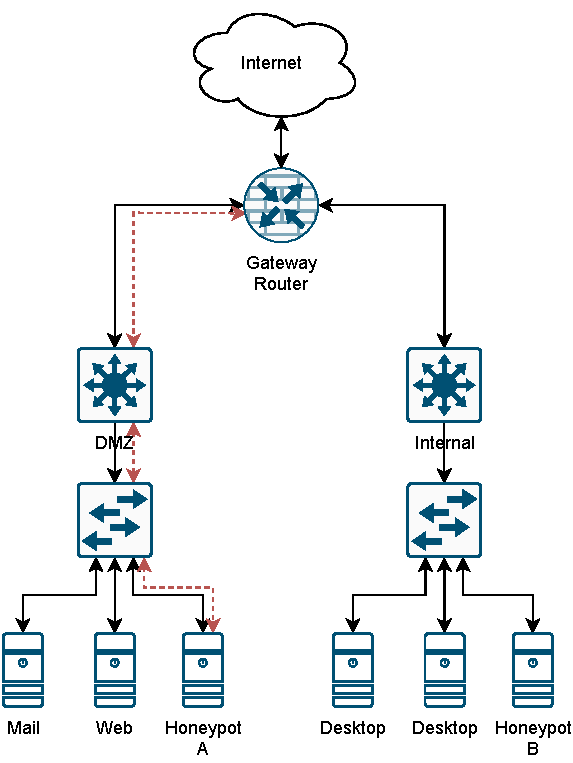
\includegraphics[width=0.5\columnwidth]{img/honeypot-example.pdf}
        \caption[Example of honeypots in a network]{
            Example of honeypots in a network (derived from \cite{Spitzner2003}).
        }
    \end{figure}
\end{frame}

\begin{frame}{T-Pot}
    \begin{columns}
        % Column 1
        \begin{column}{0.5\textwidth}
            \begin{itemize}
                \item Combines 20 honeypots for different usages
                \item Data visualization with the ELK stack
                \item High security standards
            \end{itemize}
        \end{column}
        % Column 2    
        \begin{column}{0.5\textwidth}
            \begin{figure}
                \centering
                
\includegraphics[width=\columnwidth]{img/tpot.png}
            \end{figure}
        \end{column}
    \end{columns}
\end{frame}